\documentclass[12pt]{article}
\usepackage{geometry}                % See geometry.pdf to learn the layout options. There are lots.
\geometry{letterpaper}                   % ... or a4paper or a5paper or ... 
\usepackage{graphicx}
\usepackage{amssymb}
\usepackage{amsthm}
\usepackage{epstopdf}
\usepackage[english, german]{babel}
\usepackage[utf8]{inputenc}
\usepackage[usenames,dvipsnames]{color}
\usepackage[table]{xcolor}
\usepackage{hyperref}
\DeclareGraphicsRule{.tif}{png}{.png}{`convert #1 `dirname #1`/`basename #1 .tif`.png}

\theoremstyle{definition}
\newtheorem{example}{Example}

\newenvironment{explanation}{%
   \setlength{\parindent}{0pt}
   \itshape
   \color{blue}
   \normalfont
}{}

\newcommand{\projectname}{Template}
\newcommand{\productname}{Dahoam}
\newcommand{\projectleader}{I. Gattringer}
\newcommand{\documentstatus}{In process}
%\newcommand{\documentstatus}{Submitted}
%\newcommand{\documentstatus}{Released}
\newcommand{\version}{V. 1.0}

\begin{document}
\begin{titlepage}
\begin{flushright}

\includegraphics[scale=.5]{htlleondinglogo.png}\\
\end{flushright}

\vspace{10em}

\begin{center}
{\Huge System Specification} \\[3em]
{\LARGE \productname} \\[3em]
\end{center}

\begin{flushleft}
\begin{tabular}{|l|l|}
\hline
Project Name & \projectname \\ \hline
Project Leader & \projectleader \\ \hline
Document state & \documentstatus \\ \hline
Version & \version \\ \hline
\end{tabular}
\end{flushleft}

\end{titlepage}
\section*{Revisions}
\begin{tabular}{|l|l|l|}
\hline
\cellcolor[gray]{0.5}\textcolor{white}{Date} & \cellcolor[gray]{0.5}\textcolor{white}{Author} & \cellcolor[gray]{0.5}\textcolor{white}{Change} \\ \hline
November 03, 2019&P. Bauer&First version \\ \hline
\end{tabular}
\pagebreak

\tableofcontents
\pagebreak

\section{Initial Situation and Goal}  
An Initial prototype of Dahoam was built between 2018 and 2019. The reasons for carrying out the project was to enhance the mirror in all aspects. It is in interest of the headmaster and head of department of HTL Leonding to have a project like Dahoam which represents most of the technical focuses of the school. \newline
Furthermore, Dahoam combines a smart home hub with a mirror, which can be found in most households already. \newline
To ensure privacy and security, all services of Dahoam run locally, which means no camera and voice data will be sent to the cloud.

\subsection{Initial Situation}
Since Smart Homes are getting more popular in the last few years, a big new market has appeared. Today’s situation is that devices which are managing all the different gadgets and other appliances in houses are needed. In most smart homes there is a small tablet which can be mounted on a wall in the entrance room. Which means an extra space is wasted. Dahoam should prevent the waste of extra space and combine a commercial mirror with a smart home hub, despite that a mirror is way more flexible in where to install it.

\subsubsection{Application Domain}
Dahoam is embedded in a special mirror which is most likely placed in households. The mirror handles user interaction with three services, including \textit{"Text-To-Speech"}, \textit{"Speech Recognition"} and \textit{"Intent Parser"}. Besides it recognizes people in front of it via \textit{"Face Recognition"}.

\subsubsection{Glossary}

\begin{flushleft}
\begin{tabular}{|l|l|}
\hline
Text-To-Speech & Converts output to spoken words\\ \hline
Speech Recognition & Converts spoken input to text\\ \hline
Intent Parser & Parses input to executable commands\\ \hline
Face Recognition & Compares faces in front of the camera with saved faces\\ \hline
\end{tabular}
\end{flushleft}

\subsubsection{Model of the Application Domain}
\begin{explanation}

\end{explanation}

\pagebreak
\subsection{Goal}
Dahoam should give the customer a solid smart home hub integrated in a common mirror. The intelligent mirror will run 24/7 and is only active when a person is in front of it. If there is one, a movement sensor will wake up all services. \\
Each user can have its own account, delete and personalize it. The general configuration can be edited by an administrator in Dahoam-Connect-App.

\pagebreak

\section{Functional Requirements}
In order to fulfill all requirements of a proper smart home hub the user can always get information about weather, calendar, current states of temperatures and lighting in different rooms. To show personalized data the user must be registered, which can be done through Dahoam-Connect-App. Within the app are possibilities to add calendars and email accounts. Besides of that the region for the weather forecast can be selected and other smart home devices can be added.


\subsection{Overview}
\begin{center}
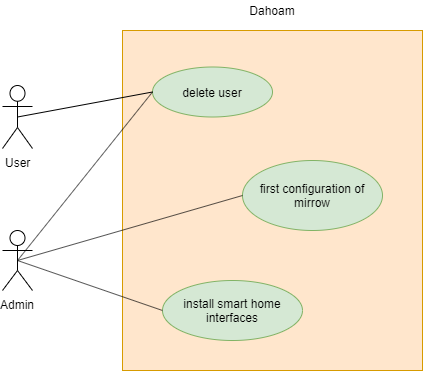
\includegraphics[scale=.7]{UseCase/UseCase.png}\\
\end{center}

\subsection{Use Case 1: $<$Delete User$>$}
\subsubsection{General Description}
In the user settings exists a "delete" button which deletes all related user data.
\\
\\
\begin{tabular}{|p{.2\linewidth}|p{.65\linewidth}|}
\hline 
ID: & Delete User/Admin \\ \hline
Goal: & The user wants to be able to delete his own account. \\ \hline
Precondition: & The use case will be triggered by pressing the "delete" button in the Dahoam-Connect-App. \\ \hline
Postcondition: & The user is deleted and will not be recognized by the mirror anymore. Also the user will not be able to log in with the deleted account in the app. \\ \hline
Involved Users: & Role name: user, admin  \\ \hline
\end{tabular}

\subsubsection{UI to call the use case}
This is the design of the user settings, where a button will be added, to be able to delete the account logged in.

\begin{center}
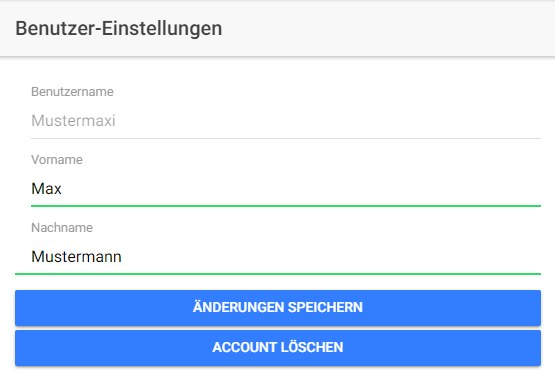
\includegraphics[scale=.8]{UseCase/DeleteUserFirstStep.PNG}\\
\end{center}
\subsubsection{The Standard Use}
The user clicks the button and his account will be deleted. The app will automatically log out the account and the mirror does not recognize the user again.
 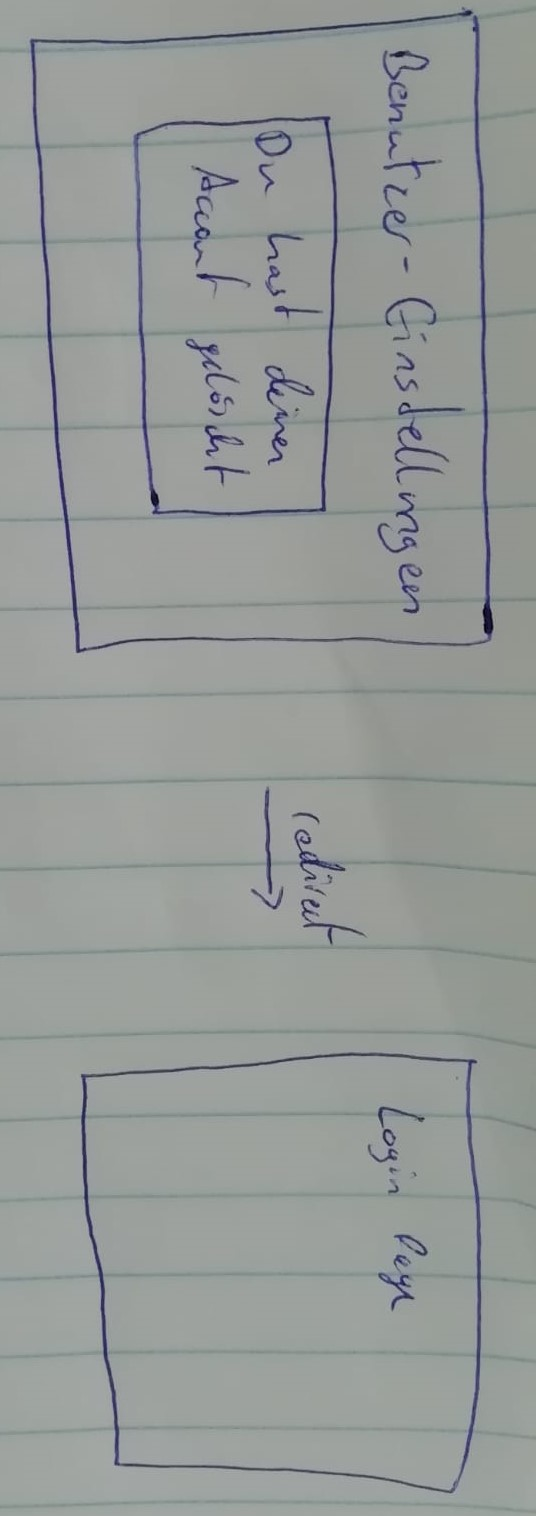
\includegraphics[angle=90, scale=.3]{UseCase/UIDELETEUSER2.png}\\

\subsubsection{The Non-Standard Use}
If the last admin for the mirror wants to delete himself, an error message must occur, because without an admin, the mirror can not change the smart home interfaces.\\\\
 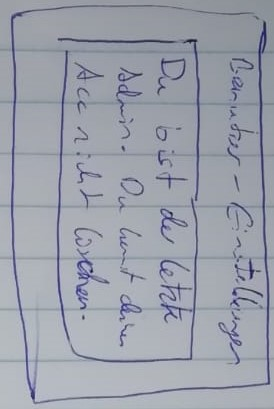
\includegraphics[angle=90, scale=.5]{UseCase/LetzterAdminWillAccountLoschen.jpeg}\\

\subsection{Use Case 2: $<$First Configuration of the Mirror$>$}
\subsubsection{General Description}
\begin{tabular}{|p{.2\linewidth}|p{.65\linewidth}|}
\hline 
ID: & Fist Configuration of mirror \\ \hline
Goal: & After the mirror has been installed, it must be configured, so that the mirror knows in which network it works.\\ \hline
Precondition: & Directly after installing the mirror this usecase will be triggered. \\ \hline
Postcondition: & The mirror knows in which network it has to operate. \\ \hline
Involved Users: & Role name: admin \\ \hline
\end{tabular}

\subsubsection{UI to call the use case}
\begin{center}
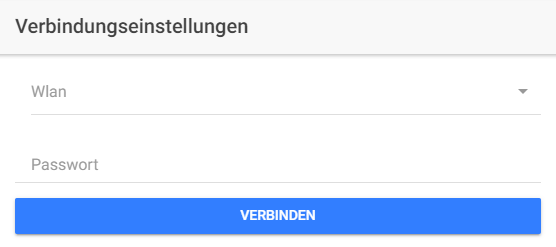
\includegraphics[scale=.8]{UseCase/StandartWlanEinstellungen.PNG}\\
\end{center}

\subsubsection{The Standard Use}
A WiFi is found and the correct password was submitted.\\\\
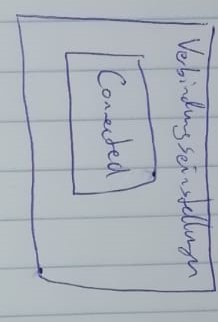
\includegraphics[angle=90, scale=.8]{UseCase/VerbindungHergestelltMitInternet.jpeg}\\

\subsubsection{The Non-Standard Use}
If there is no WiFi to connect to, the mirror cannot fulfill its main purpose - being a smart home hub.
Therefore a error message will be shown to the user. Also he will not be able to continue in the process configuring the mirror until it is connected to a WiFi.\\
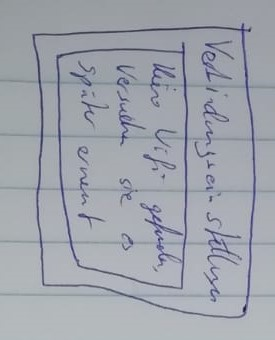
\includegraphics[angle=90, scale=.8]{UseCase/KeinWifiGefunden.jpeg}\\\\
If a WiFi got selected, but the user entered a wrong password, an alert will appear to communicate this to the user.\\\\
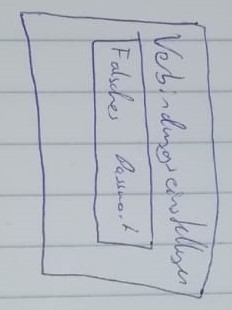
\includegraphics[angle=90, scale=.8]{UseCase/VerbindungFalschesPasswort.jpeg}\\


\subsection{Use Case 3: $<$Install Smart Home Interfaces$>$}
\subsubsection{General Description}
Connecting Smart Home Devices to the mirror with the help of MQTT. \\s
\\
\begin{tabular}{|p{.2\linewidth}|p{.65\linewidth}|}
\hline 
ID: & Install Smart Home Interfaces\\ \hline
Goal: & Connecting the mirror with smart home devices.\\ \hline
Precondition: & Admin presses the button for installing the interfaces.\\ \hline
Postcondition: & The mirror knows all different smart home devices which are installed. \\ \hline
Involved Users: & Role name: admin  \\ \hline
\end{tabular}

\subsubsection{UI to call the use case}
\begin{center}
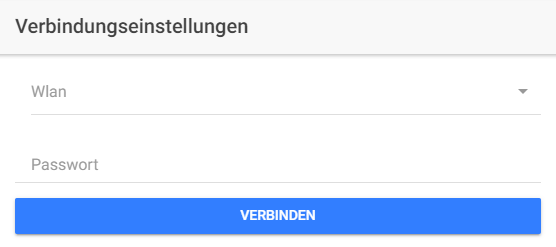
\includegraphics[scale=.8]{UseCase/StandartWlanEinstellungen.PNG}\\
\end{center}

\subsubsection{The Standard Use}
First, a MQTT broker has to be set in the Dahoam-Connect-App. After pressing the connect button a small alert will be displayed. When connected, devices can be added. First a list of all existing devices will be displayed with an add button at the bottom. When a Publication is added it is needed to specify a name as well as the topic, QoS and retained are optional. To finish the procedure it is necessary to select a type, which defines what type of values will be sent. Subscription is more or less the same, but there has to be set the name and topic since data will be received.
\begin{explanation}
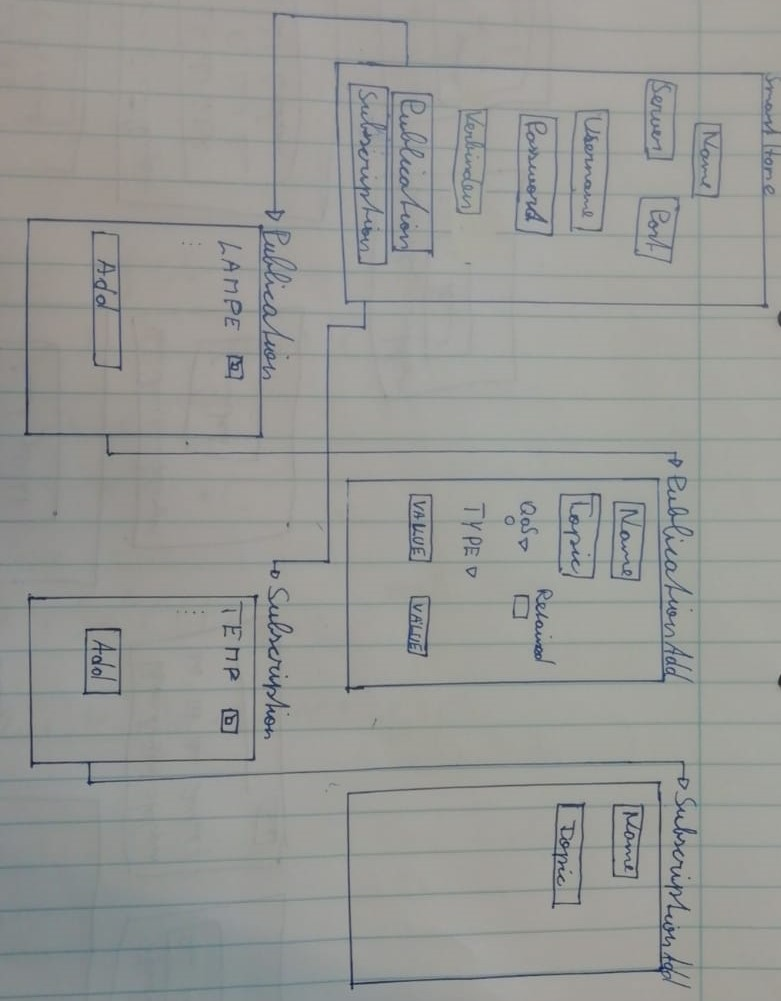
\includegraphics[angle=90, scale=.5]{UseCase/InstallSmartHomeInterfaces.jpeg}\\
\end{explanation}

\subsubsection{The Non-Standard Use}
When the user does not enter the right credentials for the broker, an alert occurs and warns him.


\pagebreak

\section{Non-Functional Requirements}
\subsection{NFR 1: Enable full Dockerized Runtime Environment}
\begin{tabular}{|p{.2\linewidth}|p{.65\linewidth}|}
\hline 
ID: & Runtime Environment \\ \hline
Name: & Enable full Dockerized Runtime Environment \\ \hline
Type	: & USE\\ \hline
Description: & It is really complicated and takes a lot of time to install all required software and programming languages on the Raspberry Pi. Therefore, a Docker runtime environment should change this. Only by typing: docker-compose up, the mirror gets started and everything necessary will be installed.\\ \hline
\end{tabular}

\subsection{NFR 2: Development Environment}
\begin{tabular}{|p{.2\linewidth}|p{.65\linewidth}|}
\hline 
ID: & Development Environment \\ \hline
Name: & Development Environment \\ \hline
Type	: & MAINT\\ \hline
Description: & Each docker-container can be tested isolated. Also the logging will be improved, so that the log level can be changed and the masterservice does not log unnecessary things as now.\\ \hline
\end{tabular}

\subsection{NFR 3: Alternative to QR-Code}
\begin{tabular}{|p{.2\linewidth}|p{.65\linewidth}|}
\hline 
ID: & Alternative to QR-Code \\ \hline
Name: & Alternative to QR-Code \\ \hline
Type	: & USE\\ \hline
Description: & Sometimes the QR-Code for registering a new user, does not work because the light outside is too bright and the phone therefore cannot scan the QR-Code. Thus, a alternative to the QR-Code is required.\\ \hline
\end{tabular}

\subsection{NFR 4: Admin Account}
\begin{tabular}{|p{.2\linewidth}|p{.65\linewidth}|}
\hline 
ID: & Admin Account \\ \hline
Name: & Admin Account \\ \hline
Type	: & USE\\ \hline
Description: &  Currently no users can be deleted and there is nobody who can manage the integration of other smart home devices. An admin can also view all registered users.\\ \hline
\end{tabular}

\subsection{NFR 5: User Administration}
\begin{tabular}{|p{.2\linewidth}|p{.65\linewidth}|}
\hline 
ID: & User Administration \\ \hline
Name: & User Administration \\ \hline
Type	: & USE\\ \hline
Description: & A user can delete his account and all related data to him. \\ \hline
\end{tabular}

\subsection{NFR 6: Demo Mode}
\begin{tabular}{|p{.2\linewidth}|p{.65\linewidth}|}
\hline 
ID: & Demo Mode \\ \hline
Name: & Demo Mode \\ \hline
Type	: & EFFIC\\ \hline
Description: & After a random amount of time some services stop working. To ensure a 24/7 runable system there is the need of a sleep mode which shuts services down when they are not needed. \\ \hline
\end{tabular}

\subsection{NFR 7: Dahoam-Flows}
\begin{tabular}{|p{.2\linewidth}|p{.65\linewidth}|}
\hline 
ID: & Dahoam-Flows \\ \hline
Name: & Dahoam-Flows \\ \hline
Type	: & USE\\ \hline
Description: & When speaking to the mirror it often understands wrong things. E.g.: "Schalte das Licht in Raum 2 und 3 ein" then it adds the two numbers and turns on the light in room 5. Furthermore a problem occurs when several registered users are in front of the mirror because it can not decide which of them should be logged in. When an unregistered user kicks off registration process and denies it, the whole registration process is blocked for the running session. While registration, a live camera feedback should help the user positioning himself in the right place.
\\ \hline
\end{tabular}


\pagebreak

\section{Quantity Structure}

Users will be saved with a username (unique), name and password, as well as a picture to identify them via the face recognition. Further more a user can add multiple email addresses and a calendar. Therefore a Database is the best option to store the master data.

\pagebreak
\section{System Architecture and Interfaces}
Dahoam is embedded whether in a common home without any smart home interfaces or in a modern home with some smart home lights or sensors installed.\\
The user is able to communicate with the mirror either with speech recognition or Dahoam-Connect-App. \\
The mirror has a connection to a weather API and has an interface to get the emails of the user by POP3. It is also capable of addressing the calendar which is saved on the phone of the user. \\


\pagebreak
\section{Acceptance Criteria}

\textbf{Delete User}\\
If a user is deleted, all related data must be removed. If a user removes his account through Dahoam-Connect-App, a confirmation message appears and the user will be redirected to the login view. If he/she is meanwhile logged into the mirror, he/she should be logged out after the deletion process. \\
\newline
\textbf{First Configuration of the Mirror}\\
The configuration must include:
\begin{itemize}
    \item Create an admin account for all further configurations
    \item Connect to an existing network (on-/offline does not matter) in order to communicate with Dahoam-Connect-App
    \begin{itemize}
        \item Online: Enter location for the weather display
    \end{itemize} 
\end{itemize}
\textbf{Install Smart Home Interfaces}\\
For configuration of smart home devices, an own page in Dahoam-Connect-App is required. Following information is required:
\begin{itemize}
    \item MQTT-Broker IP and port
    \item A username and password if needed
    \item Publish
    \begin{itemize}
        \item Name
        \item Topic
        \item QoS and retained
        \item Values
    \end{itemize}
    \item Subscription
    \begin{itemize}
        \item Name
        \item Topic
        \item QoS
    \end{itemize}
\end{itemize}
\end{document}  